R-CNN postiže dobre rezultate na problemu detekcije objekata, ali ima nekoliko velikih nedostataka. Treniranje modela je komplicirano jer se svaka komponenta trenira zasebno. Također, treniranje je vremenski i memorijski vrlo zahtjevno jer je za trening klasifikatora potrebno dobiti duboke značajke za sve slike i spremiti ih na disk što je posebno izraženo pri korištenju većih konvolucijskih mreža. Treći veliki nedostatak je sporost detekcije objekata jer je i kod predikcije potrebno za svaku predloženu regiju izlučiti duboke značajke da bi se regija mogla klasificirati.
Fast R-CNN (\cite{DBLP:journals/corr/Girshick15}) donosi nekoliko poboljšanja u odnosu na R-CNN. Cijeli model se trenira odjednom, nema potrebe za privremenim pohranjivanjem dubokih značajki i postiže veću preciznost detekcije.
Arhitektura modela prikazana je na slici \ref{fast_rcnn}. Na ulazu Fast-RCNN mreža prima sliku i skup predloženih regija u kojima se potencijalno nalazi objekt. Mreža prvo računa mapu dubokih značajki za cijelu sliku koristeći duboku konvolucijsku mrežu koja se sastoji od nekoliko konvolucijskih slojeva i nekoliko slojeva sažimanja maksimalnom vrijednošću. Nakon toga se, za svaku predloženu regiju, iz dobivene mape značajki izlučuje vektor značajki konstantne duljine korištenjem RoI (Region of Interest) sloja sažimanja. Svaki vektor značajki se zatim prosljeđuje potpuno povezanim slojevima koji se na kraju granaju u dva izlazna sloja: jedan sa softmax aktivacijskom funkcijom koji procjenjuje vjerojatnosti pripadnosti regije svakom od $K + 1$ razreda (K razreda objekata i jedan dodatni koji predstavlja pozadinu) i drugi, koji na izlazu daje četiri broja za svaki razred koji opisuju prozor u kojem se nalazi objekt. 
RoI sloj sažimanja koristi sažimanje maksimalnom vrijednošću kako bi na izlazu vratio vektor značajki konstantne veličine $H \times W$. Izlazni vektor se računa tako da se ulazni prozor dimenzija $h \times w$ podijeli u mrežu dimenzija $H \times W$, gdje je veličina svake ćelije mreže $\frac{h}{H} \times \frac{w}{W}$ te se u svakoj ćeliji odredi maksimalna vrijednost.
Važno svojstvo Fast R-CNN modela je da se sve težine mogu trenirati backpropagation algoritmom. Budući da model ima dva izlazna sloja, a ostali slojevi su dijeljeni, funkcija pogreške uključuje pogrešku oba izlazna sloja:
\[
L(p, u, t^u , v) = L_{cls}(p, u) + \lambda [u \geq 1]L_{loc}(t^u, v)
\]
gdje je $p$ vjerojatnosna razdioba na izlazu sloja sa softmax aktivacijskom funkcijom $p = (p_0, ..., p_K)$, $u$ je stvarni razred regije na ulazu, $t^k$ je predviđeni prozor, a $v$ je stvarni prozor u kojem se nalazi objekt. Izraz $[u \geq 1]$ ima vrijednost 1 ako je stvarni razred objekta neki $1...K$, a 0 ako je stvarni razred objekta 0. Razred 0 označava pozadinu pa u tom slučaju nema smisla određivati lokaciju objekta. Za pogrešku klasifikacije se koristi negativna log-izglednost stvarnog razreda $u$ $L_{cls}(p, u) = - \log p_u$, a za pogrešku lokalizacije objekta se koristi zaglađena $L_1$ pogreška
\[
L_{loc}(t^u, v) = \sum\limits_{i \epsilon \{ x, y, w, h \}} smooth_{L_1} (t^u_i - v_i)
\]
gdje je
\[
smooth{L_1}(x) = 
	\begin{cases}
		0.5x^2, \quad \quad za \quad |x| < 1 \\
		|x| - 0.5, \quad inace
	\end{cases}
\]

Funkcija pogreške koja uključuje pogreške oba izlazna sloja ima i veću preciznost u odnosu na model koji je odvojeno treniran za klasifikaciju i regresiju.
Da bi se postigla invarijantnost na skalu, koristi se metoda svođenja slika na istu skalu, gdje se skala definira kao duljina kraće stranice.
U usporedbi s R-CNNom, Fast R-CNN donosi poboljšanje u preciznosti detekcije i velika ubrzanja u treningu i detekciji objekata.

 \begin{figure}
	\centering
	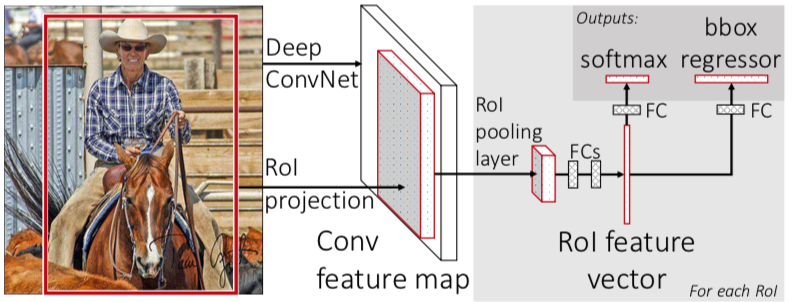
\includegraphics[scale=1]{img/fast_rcnn.png}
	\caption{Arhitektura Fast R-CNN (\cite{DBLP:journals/corr/Girshick15}).}
	\label{fast_rcnn}
\end{figure}